\subsection{基于RDMA和共享内存的环形缓冲区}
\label{socksdirect:subsec:lockless-queue}

\iffalse
\begin{figure}[t]
	\centering
	
\includegraphics[width=0.4\textwidth]{images/fixme.pdf}
	
	\caption{队列的性能比较。}
	\label{socksdirect:fig:queue-performance}
\end{figure}
\fi


\begin{figure}[htbp]
	\centering
	\subfloat[传统环形缓冲区。]{
		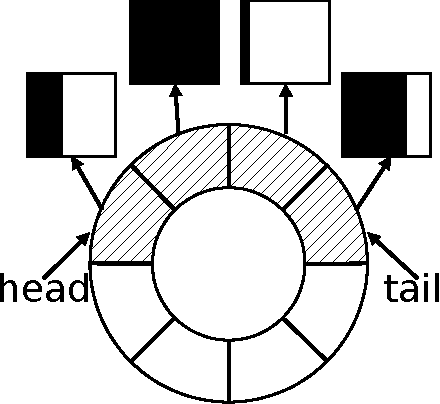
\includegraphics[width=0.3\textwidth]{images/ringbuffer_traditional}
		\label{socksdirect:fig:ringbuffer-traditional}
	}
	\hspace{0.02\textwidth}
	\subfloat[\sys 的环形缓冲区。]{
		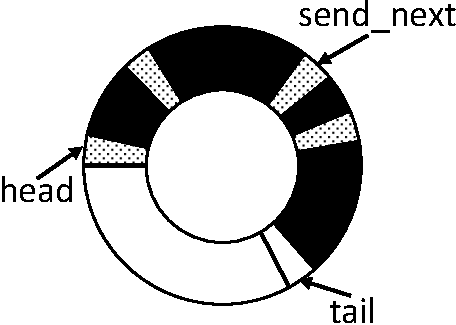
\includegraphics[width=0.32\textwidth]{images/ringbuffer_new}
		\label{socksdirect:fig:ringbuffer-new}
	}
	
	\caption{环形缓冲区数据结构。 阴影部分是元数据,黑色部分是有效载荷。}
\end{figure}


传统上,网络协议栈使用环形缓冲区从网卡发送和接收数据包。
如图 \ref {socksdirect:fig:ringbuffer-traditional} 所示,传统的环形缓冲区由一组定长的元数据构成,每个元数据指向一个定长的内存页面以存储有效载荷。这种设计会导致内存分配开销和内部碎片。
传统网卡使用这种设计的原因是环形缓冲区的数量有限,需要多个连接复用一个环形缓冲区。这种设计可以将有效载荷的元数据移动到每个连接的元数据队列,而无需复制有效载荷的内容。
幸运的是,单边 RDMA 写操作(write verb)开辟了新的设计可能性。
本章的创新是 \emph {每个套接字连接拥有专有的环形缓冲区} 并将数据包背靠背存储,如图 \ref {socksdirect:fig:ringbuffer-new} 所示。
发送方确定环形缓冲区内的偏移量(即 \emph{tail} 指针),然后使用单边 RDMA 写操作将数据包写入远程内存中 \emph{tail} 指针所指向的位置。
在传输过程中,接收端 CPU 不需要做任何事情。
当接收端应用程序调用 \texttt {recv} 操作时,数据从 \emph {head} 指针所指向的环形缓冲区位置出队。
当 \emph{head} 指针移动到与 \emph{tail} 重合时,指针指向的元数据为空,因此接收端的 \libipc{} 库能检测到队列空。
需要注意,\emph{head} 和 \emph{tail} 指针分别由接收方和发送方在本地维护,因此无需同步这两个指针。
通过共享内存传输数据的过程类似,因为共享内存和 RDMA 都支持写操作。



为了判断环形缓冲区是否已满,发送方将保持 \textit {队列信用}(queue credits)计数,指示环形缓冲区中的空闲字节数。
当发送方将数据包入队时,会消耗入队数据包大小的信用。
信用不足时,发送方会阻塞等待。
当接收方使数据包出队时,它会在本地增加计数器,并在计数器超过环形缓冲区大小的一半时,向发送方的内存中写入 \textit {信用返回标志}。发送方在检测到该标志时重新获得队列信用。
请注意,队列信用机制与拥塞控制无关;后者由网卡硬件处理 \cite {zhu2015congestion}。

\textbf {发送和接收方各有一个环形缓冲区拷贝。}
上述机制仍然需要发送端进行内存分配,因为发送方需要缓冲区来构造 RDMA 消息。
其次,上述机制不支持容器热迁移,因为 RDMA 队列中未来得及接收的剩余数据很难迁移。
第三,本章的目标是批量处理小消息以提高吞吐量。
为此,本章在发送方和接收方都保留了一份环形缓冲区的拷贝。
发送方写入其本地环形缓冲区,并调用单边 RDMA 写操作以使发送方与接收方的环形缓冲区同步。
为了最大限度地减少空闲链路上的延迟,并最大化繁忙链路上的吞吐量,本文设计了一种自适应的批处理机制(adaptive batching)。
\libipc{} 为每个环形缓冲区创建一个 RDMA 可靠连接(RC)队列对(QP),并维护一个 RDMA 消息的计数器。
如果计数器未超过阈值,则为每个套接字 \texttt {send} 操作发送 RDMA 消息。
否则,暂时不发送消息,而是用 \emph {send\_next} 标记第一个未发送的消息。
完成 RDMA 写操作后,\libipc{} 会在图 \ref {socksdirect:fig:ringbuffer-new} 中发送包含所有未发送更改的消息(从 \emph {send\_next} 到 \emph {tail})。
对于共享内存,由于高速缓存一致性(cache coherence)硬件可以自动进行核间同步,只需一个由两个进程共享的环形缓冲区 \footnote{共享内存即一个物理页面分别映射到两个进程的用户地址空间。}。

%Before sending, sender clears header of the next message to prevent the receiver from considering junk data in the ring buffer to be a message. Next, sender writes payload, then writes header, finally advances \textit{tail}. Receiver polls \textit{isvalid} at \textit{head} pointer, then copies the message, finally advances \textit{head}.
%For RDMA, the sender maintains a local copy of ring buffer, and we use one-sided RDMA write to synchronize updates from sender to receiver.
%For RDMA, it is known that one-sided verbs has higher throughput than two-sided ones; short messages has lower throughput than large ones~\cite{kalia2014using,kaminsky2016design}.
%In light of this, the inter-host queue has two identical copies in pinned sender and receiver memory, and we use one-sided RDMA write to synchronize updates from sender to receiver.
%\libipc{} polls CQ to limit the number of in-flight (sent but not acknowledged) messages, which is not only required by RDMA 网卡, but also enables \emph{adapative batching}~\cite{li2016clicknp,li2017kv}.
%When a message is enqueued to the ring buffer and the RDMA send queue is not full, it is immediately sent as an RDMA message.
%When \libipc{} polls CQ and finds an empty slot in send queue, it sends all queued but unsent data in queue as an RDMA message, because the messages are stored back-to-back in the queue.


\textbf {有效载荷和元数据之间的一致性。}
对于共享内存,英特尔和AMD的x86处理器提供了全序写入排序(total store ordering) \cite {sewell2010x86,intel-manual},这意味着每个 CPU 核观察到其他 CPU 核的写入顺序是相同的。8字节 \texttt {MOV} 指令是原子的,所以写数据包头是原子的。由于发送方在有效负载之后写入数据包头,因此接收方读取的消息是一致的,不需要内存栅栏(memory barrier)指令。

因为RDMA不能确保消息中各个部分的写入顺序 \cite {infiniband2000infiniband},确实需要确保消息完全到达再处理消息。虽然在使用go-back-0或go-back-N 丢包恢复~ \cite {dragojevic2014farm} 的RDMA网卡中,消息的写入总是顺序的,但对于具有选择性重传的更高级网卡,情况并非如此 \cite {mprdma,mittal2018revisiting}。在 \libipc {} 中,发送方使用 RDMA \textit {write with immediate}(带立即数的写)操作在接收方生成完成事件(completion event)。接收方轮询 RDMA \emph {完成队列} 而非环形缓冲区。RDMA能够确保接收方的缓存一致性,并且保证完成事件晚于数据写入 \libipc {} 环形缓冲区。


\textbf {平摊轮询开销。}
当不经常使用套接字时,轮询环缓冲区会浪费接收方的CPU周期。本章使用两种技术分摊轮询开销。
首先,对于RDMA队列,利用RDMA 网卡将事件通知复用到单个队列中。
每个线程对所有RDMA QP使用 \emph {共享完成队列},因此它只需要轮询一个队列而不是所有套接字队列。

其次,每个队列可以在\textit {轮询}(polling)和\textit {中断}(interrupt)模式之间切换。管程(monitor)的队列始终处于轮询模式。每个队列的接收方维护一个连续空轮询的计数器。当它超过阈值时,接收器向发送器发送消息,通知队列正在进入中断模式,并在短时间后停止轮询。当发送方以中断模式写入队列时,它还会通知管程,管程将通知接收方恢复轮询。

%\RED{Need a performance comparison figure of ring buffer architectures. (traditional ring buffer, new ring buffer, intra, inter, x axis: msg size, y axis: throughput)}



\subsection{零拷贝}
\label{socksdirect:subsec:zerocopy}


零拷贝的主要挑战是维持套接字API的语义。
幸运的是,虚拟内存提供了一个间接层,许多相关工作利用了这种 \emph {页面重映射}(page remapping)技术,从而可以将物理页面从发送方的虚拟地址重新映射到接收方,而不是复制。
Linux 零复制套接字 \cite {linux-zero-copy} 仅支持发送方,它的原理是将数据页设置为写时复制。
但是,许多应用程序经常在调用 \texttt{send} 后覆盖发送缓冲区,因此写时复制机制只是将复制从调用 \texttt {send} 操作的时间延迟到第一次覆盖的时间。
为了实现零拷贝接收,20年前,BSD~ \cite {thadani1995efficient} 和Solaris~ \cite {chu1996zero} 将应用程序缓冲区的虚拟页面重新映射到操作系统缓冲区的物理页面。但是,如表 \ref {socksdirect:tab:operation-performance} 所示,在现代CPU上,由于内核穿越(kernel crossing)和TLB刷新开销,重新映射一个页面的开销甚至比复制它更高。
最近,许多高性能 TCP/IP 协议栈 \cite {han2012megapipe,yasukata2016stackmap} 和 socket-to-RDMA 库 \cite {rsockets,socketsdirect} 提供标准的套接字API和备用的零拷贝API,但它们都没有实现标准API的零拷贝。
此外,没有现有的工作支持主机内套接字的零拷贝。



%A sender may write the send buffer after non-blocking \texttt{send}, and the receiver does not know the receive buffer before \texttt{recv}.
% so we can remap virtual address of a buffer to another physical page if the data occupies entire 4~KiB pages.


要启用零拷贝,需要修改网卡驱动程序以公开与页面重新映射相关的几个内核函数。
为了分摊页面重新映射成本,\libipc{} 仅对\texttt {send}或\texttt {recv}使用零拷贝,且有效载荷至少为16~KiB。
较小的消息被直接复制。

\textbf {内存对齐。}
页面重新映射仅在发送和接收地址页面对齐且传输包含整个页面时才有效。
\libipc{} 拦截\texttt {malloc}和\texttt {realloc}函数,并为大小超过 16~KiB 的内存分配操作分配4~KiB对齐的地址,因此大多数缓冲区将与页面边界对齐,而较小的内存分配按照原有方法分配,避免了内部碎片。
如果发送消息的大小不是 4~KiB 的倍数,则\texttt {send}和\texttt {recv}时将复制最后一块不是整页的数据。

有时,应用程序需要并不从分配的缓冲区起始地址开始接收或发送数据。例如,数据为 HTTP 请求的一部分,HTTP 请求的内存是对齐的,而由于 HTTP 头的存在,数据就不是对齐的了。
对于非对齐情况,如果应用程序在接收之后直接发送,而没有读写数据本身,\sys{} 也可以实现零拷贝的消息传输。\sys{} 的方法是对于非对齐的接收缓冲区,默认不执行内存拷贝,而是记录页面的映射和偏移量关系。在应用程序首次访问时通过页面异常触发数据拷贝;如果应用程序不访问数据,则无需拷贝。

%\textbf{Amortize page remapping cost.}


\textbf{减少写时复制。}
当发送方在\texttt {send}之后覆盖缓冲区时,现有设计使用写时复制(copy-on-write)。
复制是必需的,因为发送方可能会读取页面的未写入部分。
由于应用程序几乎总是将缓冲区重用于后续发送操作,因此在大多数情况下会调用写时复制,这使得零拷贝对发送方基本无用。
本文观察到,大多数应用程序不会逐字节写入发送缓冲区。 相反,它们会通过\texttt {recv}或\texttt {memcpy}覆盖发送缓冲区的整个页面,因此无需复制页面的原始数据。
对于\texttt {memcpy},\libipc{} 调用内核重新映射新页面并禁用写时复制,然后执行实际复制。
对于\texttt {recv},旧页面映射将被接收的页面替换。


\textbf {页面分配开销。}
页面重新映射机制需要内核为每个零拷贝\texttt {send}和\texttt {recv}分配和释放内存页面。
内核中的页面分配使用全局锁,这是低效的。因此,\libipc {}在本地管理每个进程中的可用页面池。
\libipc {}还跟踪收到的零拷贝页面的来源。
当页面未映射时,如果它来自另一个进程,\libipc {}会通过消息将页面返回给所有者。


\begin{figure}[htbp]
	\centering
	\subfloat[服务器内共享内存。 1)获取物理页面并设置写时复制; 2)通过共享内存发送页面地址; 3)映射收到的页面; 4)(可选)在发送方写入 / memcpy / recv时重新映射。]{
		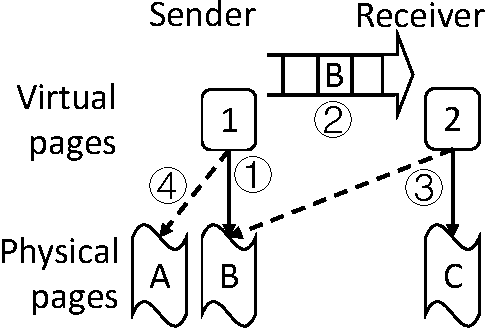
\includegraphics[width=0.44\textwidth]{images/zerocopy_intra}
		\label{socksdirect:fig:zerocopy-intra}
	}
	\hspace{0.02\textwidth}
	\subfloat[服务器间RDMA。 1)获取物理页面并设置写时复制; 2)从页面池中获取可用页面; 3)通过RDMA发送数据; 4)通过RDMA发送页面地址; 5)映射收到的页面; 6)将未映射的页面返回到页面池。]{
		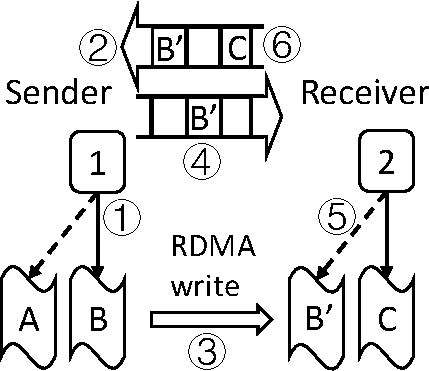
\includegraphics[width=0.42\textwidth]{images/zerocopy_inter}
		\label{socksdirect:fig:zerocopy-inter}
	}
	\caption{发送零拷贝页面的过程。}
\end{figure}


\textbf {通过共享内存安全发送页面地址。}
对于主机内部套接字,\libipc{} 在用户态队列的消息中发送物理页面地址,如图 \ref {socksdirect:fig:zerocopy-intra} 中的步骤2所示。
为了安全,\sys{} 必须防止未经发送端允许的任意页面映射。
为此,\libipc {} 调用修改后的网卡驱动程序获取发送缓冲区经过加密处理的物理页面地址,并通过共享内存队列将加密地址发送给接收方。
在接收端,\libipc {} 调用内核将加密的物理页面地址重新映射到应用程序提供的接收缓冲区虚拟地址。

\textbf {RDMA下的零拷贝。}
\libipc {} 初始化接收器上的固定页面池,并将页面的物理地址发送给发送方。
页面池由发送方管理。
在发送方上,\libipc {} 将发送缓冲区的虚拟与物理页面映射固定(pin),然后从远程接收器页面池中分配页面以确定RDMA写入的远程地址,如图 \ref {socksdirect:fig:zerocopy-inter} 中的步骤2所示。
在接收器上,当调用\texttt {recv}时,\libipc 调用网卡驱动程序将池中的页面映射到应用程序缓冲区虚拟地址。
在重新映射的页面被释放后(例如被另一个\texttt {recv}覆盖),\libipc {} 将它们返回给发送方中的页面池管理器(步骤6)。

%If the OS runs out of memory, \libipc{} unpins pages to reclaim memory.
%For security, kernel validates that page numbers are in the huge-page receive buffer.


\subsection{事件通知}
\label{socksdirect:subsec:process-mux}

\textbf {挑战1:在内核和\libipc {}之间复用事件。}
应用程序轮询来自Linux内核处理的套接字和其他\textit {内核文件描述符}的事件。
轮询内核事件的一种简单方法是每次都调用系统调用(例如\texttt {epoll\_wait}),这会产生很高的开销,因为事件轮询几乎是每次发送和接收都需调用的频繁操作。
LOS~ \cite {huang2017high} 定期用内核文件描述符调用非阻塞\texttt {epoll\_wait}系统调用,这导致延迟和CPU开销之间的权衡:如果调用太频繁,CPU 开销较高;如果调用不够频繁,则内核事件被通知到应用程序的平均延迟较高。
不同的是,\libipc {} 在每个进程中创建了一个 \textit {epoll 线程},它调用 \texttt {epoll\_wait} 系统调用来轮询内核事件。每当epoll线程收到内核事件时,应用程序线程将报告该事件以及用户空间套接字事件。

\textbf {挑战2:中断繁忙的进程。}
套接字接管机制(第 \ref {socksdirect:subsubsec:fork_rdwr} 节)需要进程响应管程请求。但是,进程可能长时间执行应用程序代码,而没有调用 \libipc {},管程请求也就无法被响应。为了解决这个问题,本章设计了一个可以类比操作系统中断的\textit {信号}(signal)机制。管程在发出请求后,首先轮询接收队列一段时间,如果超时没有回复,它会向相应进程发送 Linux \textit {信号} 并唤醒进程。

由\libipc {}注册的信号处理程序首先确定进程是执行应用程序还是\libipc {}代码。 \libipc {}在库的入口和出口处设置和清除标志。如果信号处理程序发现进程在\libipc 中,它什么也不做,\libipc {}将在将控制权返回给应用程序之前处理该事件。否则,信号处理程序会立即处理管程的消息。
因为\libipc {}被设计为快速且无阻塞(可能导致阻塞的系统调用都在 epoll 线程中调用),所以管程在发送信号后很快就会收到响应。

\textbf {挑战3:让多个线程分时核心。}
对于阻塞套接字操作(例如,阻塞recv,connect 和 epoll\_wait),\libipc {}首先轮询环形缓冲区一次。如果操作没有完成,\libipc {}调用\textit {sched\_yield}以放弃 CPU,切换到同一核心上的其他进程。如章节 \ref {socksdirect:subsec:motivation} 中所述,协同多任务处理中的上下文切换仅需要0.4~$\mu$s。但是,一些应用程序可能需要等待很长时间才能收到一个套接字消息,从而导致频繁的唤醒浪费。为此,\libipc{} 对连续的不处理任何消息的唤醒进行计数,并在达到阈值时将进程置于休眠状态。
如果\libipc {}继续产生一定数量的轮次,它将使自己进入休眠状态。在休眠之前,它会向管程和所有与之直接通信的进程(peers)发送消息,以便稍后通过信号将其唤醒。


%\textbf{Handling events from kernel.}
%An application often needs to poll kernel 文件描述符 (\textit{e.g.} files and semaphores) together with socket 文件描述符.
%\libipc{} creates a per-process \textit{epoll thread} to poll kernel 文件描述符 for all application threads. When it receives a kernel event, it broadcasts the event to application threads via shared memory queues.%\texttt{Epoll\_wait} in \libipc{} will return such kernel events in addition to socket events. Note that Linux allows an event to be received by multiple threads sharing the 文件描述符.

%\textbf{Exit.}
%When a process exits, the \texttt{atexit} handler of \libipc{} notifies the monitor and all peers to close connections and mark the queues as dead. However, a process may crash or get killed. In this case, monitor detects process death via \texttt{SIGHUP} of the bootstrap socket (Sec.~\ref{socksdirect:subsubsec:fork_fork}) and notify its peers. When a process switches to \texttt{daemon} mode or \texttt{execve} another program, it first follows the process exit procedure, then calls the system call. After that, \libipc{} is re-initialized.


\subsection{连接管理}
\label{socksdirect:subsec:connection-management}

%Before designing the connection management protocol, we keep the following requirements in mind:
%1) The applications and \libipc{} are not trusted because they are in the same memory address space. We must enforce access control policies outside \libipc{} to prevent access to restricted resources.
%2) Each address and port may be listened by multiple processes, which needs load balancing while avoid starvation.
%3) The applications may be in an overlay network and thus needs address translation. 
%%4) Multiple concurrent connections may be created between two hosts and therefore should be accelerated.
%4) A client should be able to connect to \sys{} and regular TCP/IP hosts transparently, and a server should accept connections from all hosts.

%These design requirements lead to a \emph{monitor} service running as a daemon process in each host.
%Rather than delegating all operations to the monitor, we only delegate connection creation, which forms the control plane.
%From the application's perspective, connection creation is similar to TCP handshake.
%Monitor(s) on the path between client and server applications proxy the handshake commands and help them establish a peer-to-peer queue via shared memory or RDMA.
%If the remote peer does not support \sys{}, all future operations with it will be delegated to the local monitor.
%The detailed procedure is as follows.


\subsubsection{文件描述符重映射表}
\label{socksdirect:subsubsec:fd-remapping-table}



套接字文件描述符和其他文件描述符(例如磁盘文件)共享命名空间,Linux总是分配最小的可用文件描述符。
为了保留这种语义而不在内核中分配虚拟文件描述符,\libipc {}拦截所有与文件描述符相关的Linux API并维护\emph {文件描述符重映射表}以将每个应用文件描述符映射到用户空间套接字对象或内核文件描述符。
当文件描述符关闭时,\libipc {}将其放入\emph {文件描述符回收池}。
在文件描述符分配时,\libipc {}首先尝试从池中获取文件描述符。
如果池为空,则通过递增\emph {文件描述符分配计数器}来分配新的文件描述符。
文件描述符回收池和分配计数器在进程中的所有线程之间共享。

\subsubsection{连接建立}


图 \ref {socksdirect:fig:conn-setup} 显示了连接建立过程。


\begin{figure}[htbp]
	\centering
	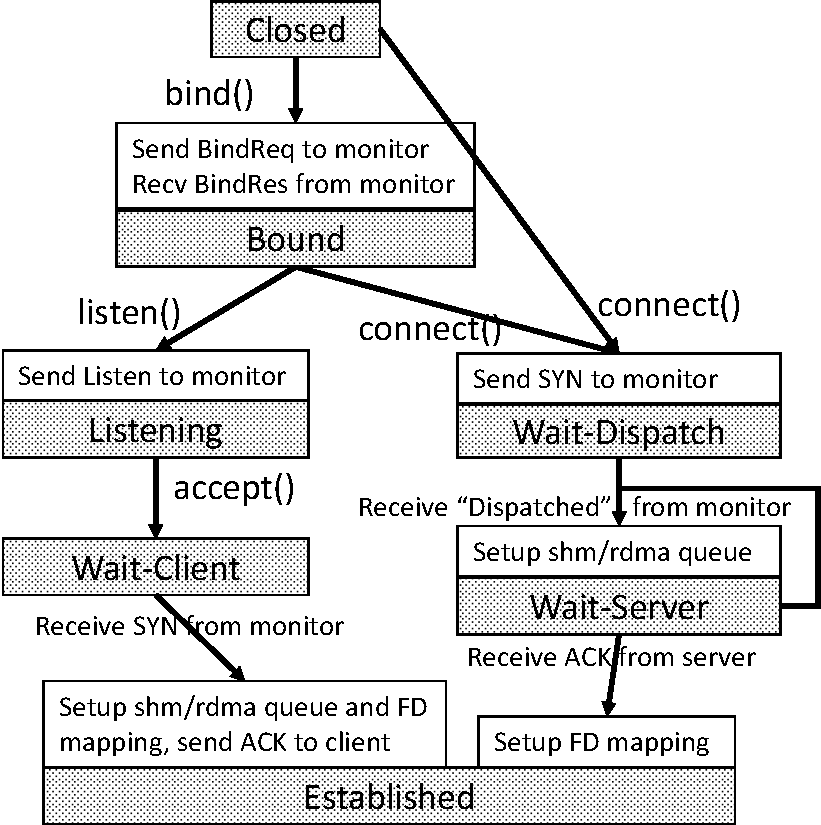
\includegraphics[width=0.6\textwidth]{images/conn-setup-new}
	\caption{\libipc{} 中连接建立过程的状态机。}
	\label{socksdirect:fig:conn-setup}
\end{figure}



\textbf{绑定。}
创建套接字后,应用程序调用\texttt {bind}来分配地址和端口。
由于地址和端口是具有权限保护的全局资源,分配由管程协调。
如图 \ref {socksdirect:fig:conn-setup} 所示,\libipc {}将请求发送到管程。
为了隐藏与管程通信的延迟,作为一个优化,如果绑定请求不可能失败(例如没有为客户端套接字指定端口时),\libipc {}会立即返回应用程序。

\textbf{监听。}
当服务器应用程序准备好接受来自客户端的连接时,它会调用\texttt {listen}并通知管程。
管程维护每个地址和端口上的监听进程列表,以分派新连接。


\textbf{连接。}
客户端应用程序调用\texttt {connect}并发送SYN命令以通过共享内存队列进行监听。
现在,管程需要将新连接分派给监听应用程序。
在Linux中,新的连接请求在内核的\emph {积压}(backlog)中排队。
每次服务器应用程序调用\texttt {accept}时,它都会访问内核以从积压中出列,这需要同步并增加延迟。
为解决此问题,\sys{} 为每个监听套接字的线程维护一个每个监听者的积压。
管程以循环方式将SYN分发给监听者线程。

当监听者不接受新连接时,分发到该监听者的连接可能会导致饥饿(starvation)。
\sys{} 使用 \emph {工作窃取}(work stealing)\footnote{工作窃取(work stealing)是实现负载均衡的一种常用方法,即每个工作者维护一个请求等待队列,当自己的队列为空时,就从其他工作者的等待队列中窃取请求。} 方法。
当监听者在积压为空时调用\texttt {accept}时,它会请求管程窃取其他人的积压。
为了避免监听者和管程之间的争用(race condition),管程向侦听器发送请求以从积压中窃取。

\textbf {建立点对点队列。}
客户端和服务器应用程序第一次通信时,服务器管程可帮助它们建立直接连接。
对于主机内部,管程分配共享内存队列并将共享内存密钥发送到客户端和服务器应用程序。
对于主机间,客户端和服务器管程建立新的RDMA QP,并将本地和远程密钥发送到相应的应用程序。
为了减少延迟,当SYN命令分发到监听者的积压时,管程会建立对等队列(peer-to-peer queue)。
但是,如果SYN被另一个监听者窃取,则需要在客户端和新监听者之间建立新队列,如图 \ref {socksdirect:fig:conn-setup} 中的Wait-Server状态所示。

\textbf {连接建立的最后步骤。}
服务器设置对等队列后,如图 \ref {socksdirect:fig:conn-setup} 左侧所示,服务器应用程序向客户端发送ACK。 ACK包含SYN请求中的客户端文件描述符及其分配的服务器文件描述符。
与TCP握手类似,服务器应用程序可以在发送ACK后将数据发送到队列。
当客户端收到ACK时,如图 \ref {socksdirect:fig:conn-setup} 右侧所示,它设置文件描述符映射并可以开始发送数据。


\subsubsection{与常规 TCP/IP 对端的兼容性}


为了与不支持\sys {}和RDMA的对等端兼容,需要检测\sys {}功能并回退到TCP/IP。
但是,Linux普通套接字不支持向TCP SYN和ACK数据包添加特殊选项。
由于中间盒(middlebox)和网络重新排序,使用另一个端口(例如LibVMA~ \cite {libvma} 的做法)也是不可靠的。
为此,\libipc{} 首先使用内核原始套接字(raw socket)直接发送带有特殊选项的SYN和ACK数据包,如果不存在特殊选项,则回退到内核TCP/IP套接字。

在客户端,管程通过网络发送带有特殊选项的TCP SYN数据包。
如果对端具有\sys {}能力,则其管程将接收特殊SYN并且知道客户端具有\sys {}能力。
然后,服务器使用特殊选项响应SYN + ACK,包括设置RDMA连接的凭据,以便两个管程之后可以通过RDMA进行通信。
如果客户端或服务器管程发现对端是常规TCP/IP主机,它将使用 Linux 的 TCP连接修复功能 \cite {tcp-connection-repair} 在内核中创建已建立的TCP连接。
然后管程通过Unix域套接字(Unix domain socket)将内核文件描述符发送到应用程序,\libipc {}可以使用内核文件描述符进行未来的套接字操作。


一个棘手的问题是接收的数据包被同时传递到原始套接字和内核网络协议栈,此时内核将回复RST数据包,因为此连接在内核中不存在。
为避免此行为,管程会安装 \emph {iptables} 规则来过滤此类出站RST数据包。



\subsubsection{连接关闭}



当应用程序调用\texttt {close}时,\libipc {}会从重映射表中删除文件描述符。
然而,套接字可能仍然有用,因为文件描述符可以与其他进程共享,并且缓冲区中可能存在未发送的数据。
\libipc{} 跟踪每个套接字的引用计数,在fork时递增,在close时递减。
为了确保未发送的数据已经发送到对端,连接关闭过程中需要在对端之间进行握手,类似于TCP close。
因为套接字是双向的,所以\texttt {close} 相当于在发送和接收方向上分别执行 \texttt {shutdown}。
如图 \ref{socksdirect:fig:conn-close},当应用程序关闭连接的一个方向时,它会向对端发送 \emph {shutdown message}(关闭消息)。
对端以关闭消息响应。
当\libipc {}在两个方向上都收到关闭消息时,将删除套接字。


\begin{figure}[htbp]
	\centering
	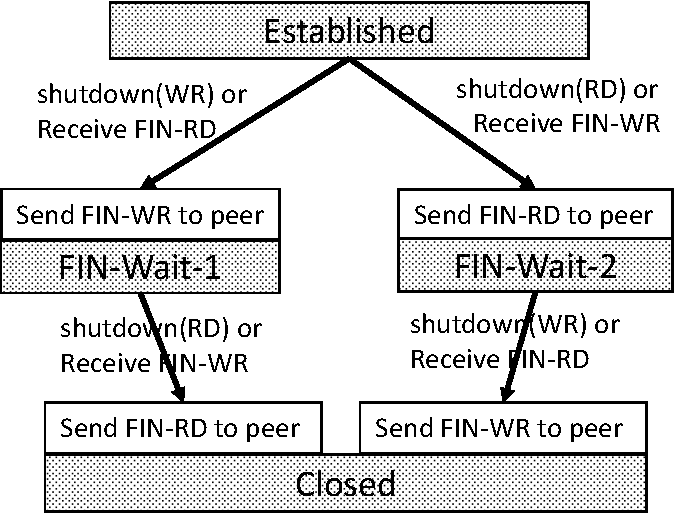
\includegraphics[width=0.5\textwidth]{images/conn-close-new}	
	\caption{\libipc{} 中连接关闭的状态机。}
	\label{socksdirect:fig:conn-close}
\end{figure}


\iffalse

\textbf{\texttt{Bind} and \texttt{listen}.}
A \emph{server} process \texttt{bind}s a socket and needs to detect IP and port conflict. In this case, \texttt{bind} is non-partitionable and goes to the monitor. The monitor also listens on the IP and port in a user-space TCP/IP stack (\textit{e.g.} mTCP~\cite{jeong2014mtcp}, LibVMA~\cite{libvma} or Seastar~\cite{seastar}) to receive connections from other hosts.

A \emph{client} process typically \texttt{bind}s without specifying IP and port, so we need to allocate a unique IP and port for it. For scalability, we partition the loopback IP address space (127.0.0.0/8) and each process allocates IP and port in its range.

\textbf{\texttt{Connect} and \texttt{accept}.}
When a client process connects to a server process on the same host, it sends a \textit{connect request} to the monitor via shared memory queue. When the server process is on another host, it creates a \textit{bootstrap TCP socket} with a special option via the user-space TCP/IP stack. If the server host supports the option, it is a \sys host and its monitor establishes an RDMA connection to the client to speedup later communications. Otherwise, the client process keeps using the bootstrap TCP socket for compatibility.

On a server host, the monitor distributes connect requests to server processes in a round-robin order, and a \textit{backlog} is maintained in each process. If the client is TCP only, the monitor proxies messages between the server process and the user-space TCP/IP stack. If the client is intra-server or RDMA capable, and it is the first time for the client and server processes to communicate, the monitor creates an inter-process queue for the process pair and sends the credentials to both processes via bootstrap sockets. After a server process \texttt{accept}s a connection in the backlog, it sends a message to the client via inter-process queue to create an 文件描述符 mapping, then the socket is ready for data transmission. As Figure~\ref{socksdirect:fig:conn-setup} shows, connection creation takes three inter-process delays.

Distributing connection to listeners may lead to starvation when a listener does not \texttt{accept} new connections. We devise a \textit{work stealing} approach. When a listener \texttt{accept}s from empty backlog, it requests the monitor to steal from others' backlog. To avoid polling empty backlogs, each listener notifies the monitor when its backlog becomes empty. To avoid contention between a listener and monitor, the monitor sends a request to the listener rather than stealing from the backlog directly.

%\subsubsection{Connection Close}

\textbf{\texttt{Close} and \texttt{shutdown}.}
Connection close is a peer-to-peer operation because only the peer process needs to be notified. If 文件描述符 is deleted immediately after \texttt{close}, a new connection may reuse the 文件描述符 while the peer process might not yet have received the close event thus sends data to the wrong connection. To avoid this, we require a handshake between peers.
Because socket is bidirectional, \texttt{close} is equivalent to \texttt{shutdown} on both send and receive directions.
When application shuts down one direction of a connection, it sends a \textit{shutdown message} to the peer. The peer responds with a shutdown message. A process deletes an 文件描述符 when it receives shutdown messages in both directions.

%In order to achieve high scalability, we separate scalable operations to different processes. To avoid the overhead of contention, \libipc enable the file descriptor allocation by individual process and when a connection is setup, the other peer of the connection gets notified of the file descriptor number by message passing. Since we treat different threads in one process as different processes, we allocate file descriptor of different ranges to each of them to avoid collision. Since file descriptor is managed separately by each process, it is possible that a file descriptor is reused after the connection is closed. Our solution is that resources of a file descriptor is not released until an ACK is received for the close operation.

%Generally, each process in our design is treated as an endpoint in the network. Figure \ref{socksdirect:fig:conn-setup-close} shows the process of connection setup and close. When \textit{socket} is called, the process itself allocate per fd resources. When \textit{listen} is called, monitor is notified of port occupation. During the \textit{connect} operation, monitor first chooses one of the processes listen on this port then coordinates the creation of the shared memory between the two processes and notifies each other of the new connection. When \textit{close} happens, both of the endpoint notify each other and monitor is responsible to destroy the shared memory between them. 

\fi
